\documentclass[aspectratio=169, table]{beamer}

\usepackage{array}
\usepackage{colortbl}
\usepackage{tabularx}
\usepackage{booktabs}
\usepackage{adjustbox}
\usepackage{xcolor}
\usepackage{tikz}
\usetikzlibrary{arrows.meta, positioning, calc, fit}

\makeatletter
\def\input@path{{../theme/}}
\makeatother
\graphicspath{{../theme/}{../../paper/figures/}}
\usetheme{Pradita}

% ---- helpers (match the template's style) ----------------------------------
\newcommand{\sectionframe}[1]{%
  \begin{frame}{\hfill}
    \centering
    \Huge{\textbf{#1}}
  \end{frame}
}
\newcommand{\takeaway}[1]{%
  \vspace{3pt}
  {\footnotesize #1}
}
% greener / winner highlight
\newcommand{\best}[1]{\textbf{\color{praditagreen}#1}}
% table wrapper: black rules + auto-fit (never clips / overflows)
\newenvironment{fittable}[1][0.66]
  {\begin{center}\arrayrulecolor{black}\footnotesize
   \begin{adjustbox}{max width=\linewidth,max totalheight=#1\textheight}}
  {\end{adjustbox}\end{center}}

% RQ callout: green border, no shadow (tcolorbox has no shadow by default)
\newtcolorbox{rqbox}{colframe=praditagreen, colback=praditagreen!6,
  boxrule=0.6pt, arc=1mm, left=2mm, right=2mm, top=1mm, bottom=1mm,
  title=Research question, fonttitle=\footnotesize\bfseries,
  coltitle=white, colbacktitle=praditagreen, before skip=3pt, after skip=3pt}

\subtitle{The 10th International Conference on Applying New
Technology in Green Buildings $\cdot$ ATiGB 2026}
\title{Carbon Footprint of Document-\\[1pt]
  Oriented vs. Relational Storage\\[1pt] 
  for Image-Based Time-Series\\[1pt] 
  Workloads\\[1pt]
}
\author{\textbf{Alfa Yohannis}, A. Waworuntu, E. Siregar, A. Sanjaya, R. Avrianto}
\date{Da Nang, Vietnam $\cdot$ 10--11 July 2026}

\begin{document}

\frame{\titlepage}

\begin{frame}{Contents}
  \vspace{12pt}
  \begin{columns}[t]
    \column{0.5\textwidth}
    \tableofcontents[sections={1-2}]
    \column{0.5\textwidth}
    \tableofcontents[sections={3-4}]
  \end{columns}
\end{frame}

% ============================================================
\section{Motivation}
\sectionframe{Motivation}

\begin{frame}{Storage is a carbon choice}
  \vspace{2pt}
  \footnotesize
  \begin{itemize}\setlength{\itemsep}{3pt}
    \item Smart buildings store IoT (Internet of Things) camera images (1080p--5K) \textbf{inline with timestamps}, in a data tier that runs \textbf{24/7} --- its energy is operational carbon.
    \item Two general-purpose engines, \textbf{opposite designs} for the binary payload:
      \begin{itemize}\footnotesize
        \item \textbf{PostgreSQL/TimescaleDB} --- TOAST (The Oversized-Attribute Storage Technique) relocates large \texttt{BYTEA} values \emph{out-of-line}.
        \item \textbf{MongoDB} time-series --- stores the image \emph{inline} as BSON (Binary JSON) \texttt{BinData} (WiredTiger + Snappy).
      \end{itemize}
    \item Existing time-series benchmarks use \textbf{tiny numeric payloads} and \textbf{report no energy}.
  \end{itemize}
  \vspace{2pt}
  \begin{rqbox}\footnotesize What is the carbon footprint of inline image storage in \textbf{PostgreSQL vs.\ MongoDB} across camera resolutions, and which engine is greener for IoT building monitoring?
  \end{rqbox}
  \takeaway{The storage backend is a \textbf{sustainability} decision, not only a performance one.}
\end{frame}

% ============================================================
\section{Approach \& Setup}
\sectionframe{Approach \& Setup}

\begin{frame}{Two architectures}
  \vspace{20pt}\footnotesize

  \centering
  \begin{adjustbox}{scale=1.2}
    \begin{tikzpicture}[font=\scriptsize, node distance=2.4mm,
        hd/.style={rounded corners=1mm, align=center, minimum width=33mm, minimum height=7mm, font=\scriptsize\bfseries, text=white},
        box/.style={draw, rounded corners=1mm, align=center, minimum width=33mm, minimum height=9mm},
        meta/.style={box, fill=gray!12}]
      \node[hd, fill=blueColor] (pgh) {PostgreSQL (PG)};
      \node[meta, below=of pgh] (pgm) {row:\\ metadata + pointer};
      \node[box, fill=blueColor!16, draw=blueColor, below=of pgm] (toast) {TOAST\\ image out-of-line};
      \draw[-Latex] (pgm)--(toast);
      \node[hd, fill=praditagreen, right=9mm of pgh] (mgh) {MongoDB (MG)};
      \node[meta, below=of mgh] (mgm) {document:\\ metadata};
      \node[box, fill=praditagreen!16, draw=praditagreen, below=of mgm] (bin) {inline BinData\\ image in document};
      \draw[-Latex] (mgm)--(bin);
    \end{tikzpicture}
  \end{adjustbox}

  \takeaway{Only the storage engine differs --- everything else is held constant.}

  \begin{columns}[T]
    \column{0.6\textwidth}\centering
    \begin{itemize}\setlength{\itemsep}{3pt}
      \item \textbf{Identical workload}
      \item 4 resolutions: \textbf{1080p--5K} (quality-90 JPEG [Joint Photographic Experts Group], 0.80--5.09~MB).
      \item 2{,}000 records, batches of 50, \textbf{5 insert runs} $+$ \textbf{5 retrieval runs}.
    \end{itemize}

    \column{0.4\textwidth}
    \begin{itemize}\setlength{\itemsep}{3pt}
      \item Storage amplification $=$ on-disk $\div$ raw payload.
      \item Both wiped/rebuilt between resolutions; compound index on device $+$ timestamp.
    \end{itemize}
  \end{columns}
\end{frame}

\begin{frame}{Measurement environment}
  \vspace{2pt}
  \footnotesize
  \begin{columns}[t]
    \column{0.52\textwidth}
    \begin{itemize}\setlength{\itemsep}{2.5pt}
      \item Single host: \textbf{Intel Core i9-11900H}, 31~GB random-access memory (RAM), 1.9~TB NVMe (Non-Volatile Memory Express) solid-state drive (SSD).
      \item Energy via \textbf{Intel RAPL} (Running Average Power Limit) counters (central processing unit [CPU] $+$ memory, machine mode) through \textbf{CodeCarbon}.
      \item Indonesia grid intensity $\approx$\,\textbf{0.676}~kg~CO\textsubscript{2}-equivalent (CO\textsubscript{2}eq) per kilowatt-hour (kWh).
      \item MongoDB WiredTiger cache capped at \textbf{30~GB} (nearly all RAM).
      \item Per-resolution emissions: constant power-rate estimate; \textbf{phase totals measured}.
    \end{itemize}
    \column{0.48\textwidth}
    \begin{fittable}[0.6]
    \begin{tabular}{ll}
      \toprule
      \textbf{Component} & \textbf{Version} \\
      \midrule
      Host OS    & Linux 6.8.0 (x86\_64) \\
      Docker     & Compose v2 \\
      PostgreSQL & 15 + TimescaleDB 2.x \\
      MongoDB    & 7.0 \\
      Python     & 3.14.3 \\
      CodeCarbon & 3.2.6 \\
      \bottomrule
    \end{tabular}
    \end{fittable}
    \centering{\scriptsize Table~I --- Software stack}
  \end{columns}
  \takeaway{Hardware-level energy under \textbf{identical} conditions for both engines.}
\end{frame}

% ============================================================
\section{Results}
\sectionframe{Results}

\begin{frame}{Performance summary}
  \vspace{2pt}
  \begin{fittable}[0.62]
  \begin{tabular}{l r rr rr rr}
    \toprule
     & \textbf{Raw} & \multicolumn{2}{c}{\textbf{Insert (r/s)}} & \multicolumn{2}{c}{\textbf{Retrieval (ms)}} & \multicolumn{2}{c}{\textbf{Storage amp.}} \\
    \cmidrule(lr){3-4}\cmidrule(lr){5-6}\cmidrule(lr){7-8}
    \textbf{Res.} & \textbf{(MB)} & \textbf{PG} & \textbf{MG} & \textbf{PG} & \textbf{MG} & \textbf{PG} & \textbf{MG} \\
    \midrule
    1080p & 1600  & 87.6 & \best{337.6} & 6906  & \best{2412}  & 1.04$\times$ & \best{0.10$\times$} \\
    1440p & 2800  & 49.9 & \best{128.3} & 11619 & \best{4260}  & 1.04$\times$ & \best{0.27$\times$} \\
    4K    & 5980  & \best{23.3} & 18.1  & 25267 & \best{10143} & \best{1.04$\times$} & 1.58$\times$ \\
    5K    & 10180 & \best{13.6} & 7.8   & 47044 & \best{28377} & \best{1.04$\times$} & 3.00$\times$ \\
    \bottomrule
  \end{tabular}
  \end{fittable}
  \takeaway{Insert \textbf{crossover} between 1440p and 4K; MongoDB reads faster everywhere; storage amplification diverges (MG up to \textbf{3.0$\times$} at 5K vs.\ PG's flat 1.04$\times$).}
\end{frame}

\begin{frame}{}
  \centering
  \vspace{1mm}
  
\includegraphics[height=.8\textheight,keepaspectratio]{boxplot_insert_throughput.pdf}\\
  \takeaway{MongoDB wins at 1080p ($3.85\times$) and 1440p ($2.57\times$); PostgreSQL overtakes at 4K and 5K as multi-MB BSON documents stress WiredTiger's B-tree write path.}
\end{frame}

\begin{frame}{}
  \centering
  \vspace{1mm}
  
\includegraphics[height=.8\textheight,keepaspectratio]{boxplot_retrieval_latency.pdf}\\
  \takeaway{Inline BSON co-locates the image with its metadata ($1.7$--$2.9\times$ faster reads); PostgreSQL must follow TOAST pointers to a secondary table.}
\end{frame}

\begin{frame}{Carbon breakdown}
  \vspace{2pt}
  \begin{fittable}[0.60]
  \begin{tabular}{l rr rr rr rr rr}
    \toprule
    \textbf{Res.}
      & \multicolumn{2}{c}{\textbf{Duration (s)}}
      & \multicolumn{2}{c}{\textbf{Energy (µWh)}}
      & \multicolumn{2}{c}{\textbf{CPU (µWh)}}
      & \multicolumn{2}{c}{\textbf{RAM (µWh)}}
      & \multicolumn{2}{c}{\textbf{Emis. (mg)}} \\
    \cmidrule(lr){2-3}\cmidrule(lr){4-5}\cmidrule(lr){6-7}\cmidrule(lr){8-9}\cmidrule(lr){10-11}
      & PG & MG & PG & MG & PG & MG & PG & MG & PG & MG \\
    \midrule
    1080p & 148.7 & \best{41.7}   & 1872  & \best{542}   & 1046  & \best{310}   & 826  & \best{232}  & 1266 & \best{366} \\
    1440p & 258.5 & \best{99.3}   & 3254  & \best{1290}  & 1818  & \best{739}   & 1436 & \best{552}  & 2200 & \best{872} \\
    4K    & \best{555.8} & 602.1  & \best{6997}  & 7824  & \best{3910}  & 4480  & \best{3088} & 3345 & \best{4730} & 5289 \\
    5K    & \best{973.1} & 1430.1 & \best{12252} & 18585 & \best{6845}  & 10640 & \best{5406} & 7945 & \best{8281} & 12562 \\
    \midrule
    \textbf{Total} & \best{2167} & 2378 & \best{27280} & 30906 & \best{15242} & 17694 & \best{12038} & 13212 & \best{18439} & 20891 \\
    \bottomrule
  \end{tabular}
  \end{fittable}
  \takeaway{Measured totals: PostgreSQL \best{18{,}439} vs.\ MongoDB 20{,}891~mg~CO\textsubscript{2}eq --- a \textbf{13.3\% overall advantage for PostgreSQL} (green $=$ lower per row).}
\end{frame}

\begin{frame}{}
  \centering
  \vspace{1mm}
  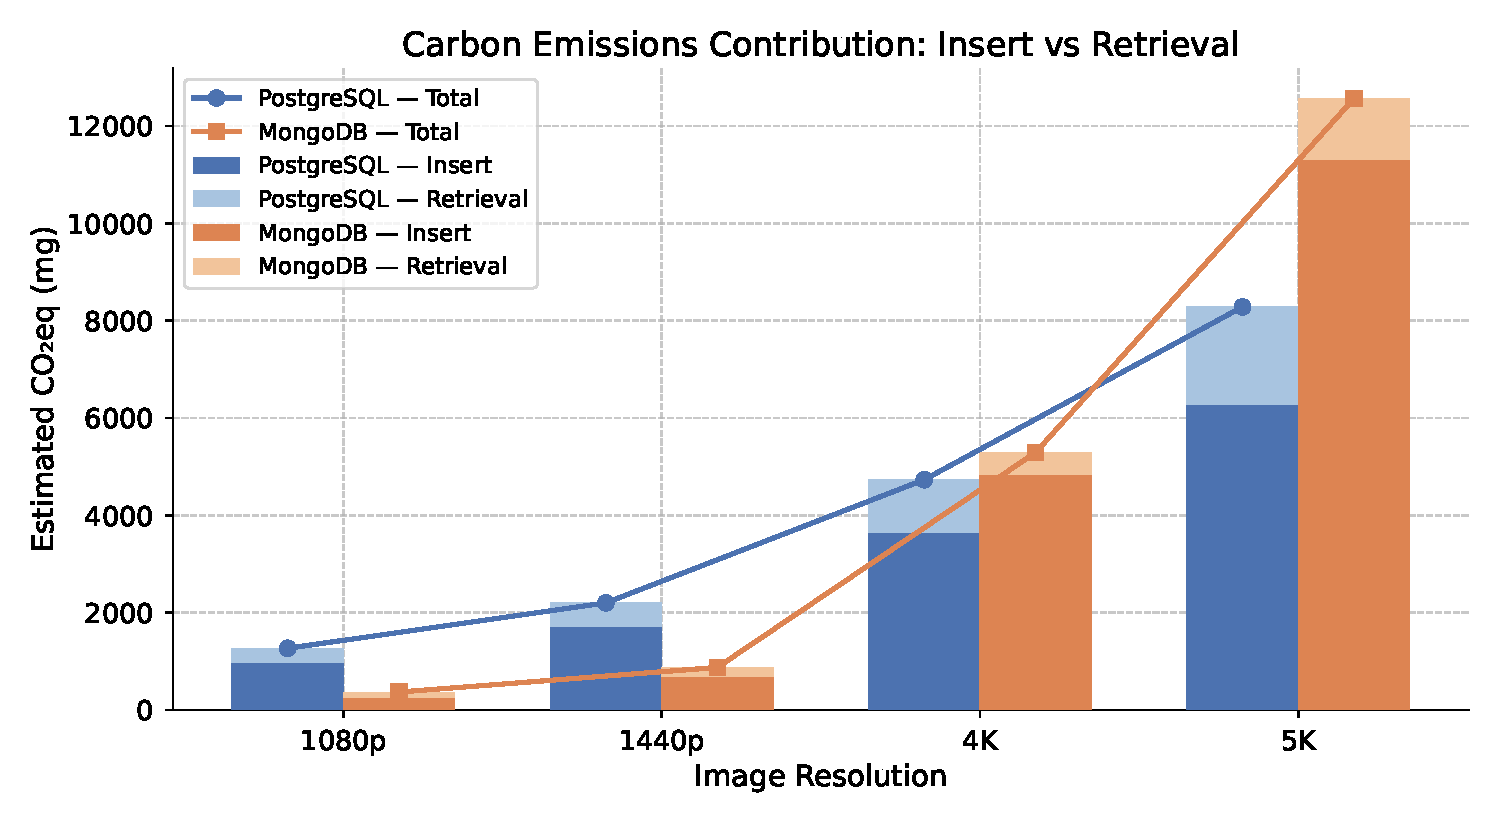
\includegraphics[height=.8\textheight]{carbon_footprint.pdf}\\
  \takeaway{MongoDB is greener at 1080p--1440p (it finishes far faster); PostgreSQL is greener at 4K--5K, where MongoDB's write amplification dominates.}
\end{frame}

\begin{frame}{}
  \centering
  \vspace{1mm}
  
\includegraphics[height=.8\textheight,keepaspectratio]{carbon_breakdown.pdf}\\
  \takeaway{CPU $\approx$57\% of energy in both; above 1440p MongoDB exceeds PostgreSQL on every component --- driven by inline BSON serialization of multi-MB payloads.}
\end{frame}

% ============================================================
\section{Discussion \& Conclusion}
\sectionframe{Discussion \& Conclusion}

\begin{frame}{Why the crossover}
  \vspace{2pt}
  \footnotesize
  \begin{columns}[t]
    \column{0.5\textwidth}
    \textbf{Mechanism}
    \begin{itemize}\setlength{\itemsep}{2pt}
      \item \textbf{MongoDB $\uparrow$ at high-res:} multi-MB BSON written inline through B-tree pages; Snappy defeated by JPEG (amp $0.10\times\!\to\!3.0\times$).
      \item \textbf{PostgreSQL efficient:} TOAST out-of-line keeps a compact, resolution-independent write path (flat $1.04\times$).
    \end{itemize}
    \column{0.5\textwidth}
    \textbf{Carbon-aware guidelines}
    \begin{itemize}\setlength{\itemsep}{2pt}
      \item $\lesssim$1.5~MB (1080p--1440p): \best{MongoDB} --- faster ingest \& reads, lower carbon.
      \item $\gtrsim$3~MB (4K$+$): \best{PostgreSQL} --- faster ingest, lower carbon, flat $1.04\times$.
      \item Read-heavy: \textbf{MongoDB} ($1.7$--$2.9\times$ faster reads).
      \item High-res sustained: \textbf{hybrid} with an object store (MinIO / Amazon S3, Simple Storage Service).
    \end{itemize}
  \end{columns}
  \takeaway{No universal winner --- choose the engine by \textbf{camera resolution}.}
\end{frame}

\begin{frame}{Conclusion}
  \vspace{2pt}
  \footnotesize
  \begin{itemize}\setlength{\itemsep}{3pt}
    \item \textbf{RQ answer:} MongoDB 20{,}891 vs.\ PostgreSQL \best{18{,}439}~mg~CO\textsubscript{2}eq --- a \textbf{13.3\% carbon premium for MongoDB} overall, driven by the 4K--5K profiles.
    \item Per-resolution: MongoDB greener $\le$1440p; PostgreSQL greener $\ge$4K. MongoDB keeps a $1.7$--$2.9\times$ \textbf{retrieval} edge throughout.
    \item \textbf{Threats:} single host; per-resolution figures are constant-power-rate estimates; 30~GB WiredTiger cache.
    \item \textbf{Future work:} hybrid metadata$+$object store (MinIO/S3); PostgreSQL Large Objects; 6K \& video; distributed deployments.
  \end{itemize}
  \takeaway{Resolution-aware, carbon-aware database selection for green IoT.}
\end{frame}

\begin{frame}{\hfill}
  \centering
  \Huge{\textbf{Thank you}}\\[8pt]
  \normalsize Questions \& discussion
\end{frame}

\end{document}
